% !TEX root = saveliev_physics_general_course_1.tex
%!TEX TS-program = pdflatex
%!TEX encoding = UTF-8 Unicode


\chapter{HYDRODYNAMICS}\label{chap:9}

\section{Streamlines and Flow Tubes. Flow Continuity}\label{sec:9_1}

Mechanics of continuous media exists in addition to the mechanics of a point particle and the mechanics of a rigid body which we treated in preceding chapters. This science covers hydrodynamics, gas dynamics, the theory of elasticity (some questions of which were dealt with in Secs.~\ref{sec:2_9} and~\ref{sec:3_8}), and a number of other branches of science considering a substance as a continuous medium. Hydrodynamics is the branch of mechanics of continuous media studying the motion of incompressible liquids and their interaction with solids.

To describe the motion of a liquid, we can set the position of each of its particles as a function of time. This method of description was worked out by J.~Lagrange. But it is also possible to observe separate points of space instead of liquid particles and record the velocity with which separate particles of the liquid pass each given point. The second method is called the Euler method.

The state of motion of a liquid can be determined by indicating the velocity vector as a function of time for each point of space. The combination of the vectors $\vec{v}$ given for all the points of space forms the so-called \textbf{velocity vector field} that can be depicted as follows. Let us draw lines in a flowing liquid so that a tangent to them at each point coincides in direction with the vector $\vec{v}$ (\fig{9_1}). These lines are called \textbf{streamlines}. We shall agree to draw the streamlines so that their density (characterized by the ratio of the number of lines $\Delta N$ to the magnitude of the area $\Delta S$ at right angles to them through which they pass) is proportional to the magnitude of the velocity at the given place. The pattern of the streamlines will thus permit us to assess not only the direction, but also the magnitude of the 	vector $\vec{v}$ at different points of space: the streamlines will be closer together where the velocity is higher and, conversely, farther apart where the velocity is lower.

Since the magnitude and the direction of the vector $\vec{v}$ may change with time at every point, then the pattern of the streamlines may also change continuously. If the velocity vector is constant at each point of space, then the flow is called \textbf{steady}. In steady flow, any particle of a liquid passes a given point of space with the same value of $\vec{v}$. The pattern of the streamlines in steady flow remains unchanged, and the streamlines in this case coincide with the trajectories of the particles.

\begin{figure}[t]
	\begin{center}
		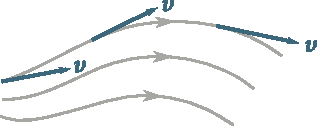
\includegraphics[scale=1.0]{figures/ch_09/fig_9_1.pdf}
		\caption[]{}
		\label{fig:9_1}
	\end{center}
	\vspace{-0.8cm}
\end{figure}

A portion of a liquid confined by streamlines is called a flow tube. The vector $\vec{v}$, being at each point tangent to a streamline, will also be tangent to the surface of the flow tube. Hence, the particles of the liquid in their motion do not intersect the ``walls'' of the flow tube.

Let us take a cross section $S$ of a flow tube (\fig{9_2}) at right angles to the direction of the velocity. We shall assume that the velocity of the liquid particles is the same at all points of this section. During the time $\Delta t$, all the particles whose distance from $S$ at the initial moment did not exceed the value $v\Delta t$ will pass through section $S$. Consequently, a volume of the liquid equal to $Sv$ will pass through section $S$ during the time $\Delta t$, and a volume of the liquid equal to $Sv$ will pass through it in unit time. Let us take a flow tube so thin that at each section of it the velocity may be considered constant. If the liquid is incompressible (\ie, its density is the same everywhere and cannot change), then the amount of liquid between sections $S_1$ and $S_2$ (\fig{9_3}) will remain constant. Hence, it follows that the volumes of liquid flowing in a unit time through sections $S_1$ and $S_2$ must be the same:
\begin{equation*}
	S_1v_1 =S_2v_2
\end{equation*}

\noindent
(we remind our reader that the particles of the liquid do not pass through the side surface of a flow tube).

\begin{figure}[t]
	\begin{minipage}[t]{0.5\linewidth}
		\begin{center}
			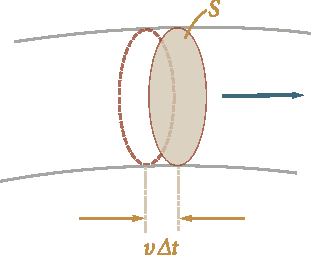
\includegraphics[scale=1.0]{figures/ch_09/fig_9_2.pdf}
			\caption[]{}
			\label{fig:9_2}
		\end{center}
	\end{minipage}
	\hspace{-0.0cm}
	\begin{minipage}[t]{0.5\linewidth}
		\begin{center}
			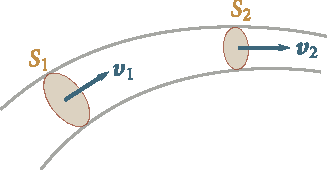
\includegraphics[scale=1.0]{figures/ch_09/fig_9_3.pdf}
			\caption[]{}
			\label{fig:9_3}
		\end{center}
	\end{minipage}
	\vspace{-0.0cm}
\end{figure}

The above reasoning may be applied to any pair of sections $S_1$ and $S_2$. Consequently, \textit{for an incompressible liquid, the quantity $Sv$ must be the same for any section of the same flow tube}:
\begin{equation}\label{eq:9_1}
	Sv = \text{constant}.
\end{equation}

\noindent
The result obtained forms the content of the theorem on \textbf{flow continuity}.

It can be seen from \eqn{9_1} that when a flow tube has a varying section the particles of an incompressible liquid will move with acceleration. In a horizontal flow tube (\fig{9_4}), this acceleration can be due only to the lack of constancy of the pressure along the axis of the tube---at places where the velocity is smaller, the pressure must be greater, and vice versa. The quantitative relation between the flow velocity and the pressure will be established in the following section.

The theorem on flow continuity can be applied to real liquids and even to gases when their compressibility may be disregarded. The relevant calculations show that when fluids flow with velocities lower than the speed of sound, they may be considered incompressible with a sufficient degree of accuracy.

\begin{figure}[t]
	\begin{center}
		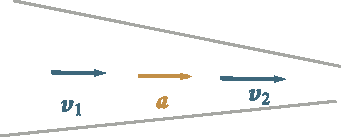
\includegraphics[scale=1.0]{figures/ch_09/fig_9_4.pdf}
		\caption[]{}
		\label{fig:9_4}
	\end{center}
	\vspace{-0.8cm}
\end{figure}

\section{Bernoulli's Equation}\label{sec:9_2}

When dealing with the motion of liquids, we can often consider that the displacement of some portions of a liquid relative to others is not associated with the appearance of forces of friction. A liquid in which internal friction (viscosity) is completely absent is called \textbf{ideal} (or \textbf{non-viscous}).

Let us separate a flow tube of small cross section (\fig{9_5}) in a steadily flowing ideal liquid. We shall consider the volume of the liquid confined by the ``walls'' of the flow tube and by cross sections $S_1$ and $S_2$ perpendicular to the streamlines. During the time $\Delta t$, this volume will move along the flow tube. Section $S_1$ will move to position $S_1'$ having covered the distance $\Delta l_1$, and section $S_2$ will move to position $S_2'$ having covered the distance $\Delta l_2$. Owing to flow continuity, the shaded volumes will be equal: $\Delta V_1 = \Delta V_2 = \Delta V$.

\begin{figure}[t]
	\begin{center}
		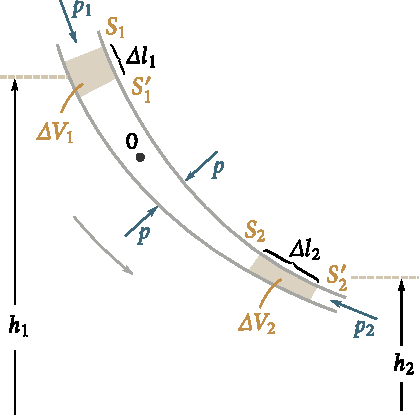
\includegraphics[scale=1.0]{figures/ch_09/fig_9_5.pdf}
		\caption[]{}
		\label{fig:9_5}
	\end{center}
	\vspace{-0.8cm}
\end{figure}

The energy of each liquid particle consists of its kinetic energy and its potential energy in the field of the Earth's gravitational forces. Owing to the steady nature of the flow, a particle that after the time $\Delta t$ is at any point in the unshaded part of the volume being considered (see, for example, point $0$ in \fig{9_5}) has the same velocity (and, consequently, kinetic energy) as the particle did that was at the same point at the initial moment. Hence, the energy increment $\Delta E$ of the entire volume being considered can be calculated as the difference between the energies of the small shaded volumes $\Delta V_1$ and $\Delta V_2$.

Let us take a flow tube cross section and the lengths $\Delta l$ so small that the same values of the velocity $v$, pressure $p$, and height $h$ can be ascribed to all the points of each of the shaded volumes. Hence, the energy increment can be written as follows:
\vspace{-12pt}
\begin{equation}\label{eq:9_2}
	\Delta E = \left(\frac{\rho\Delta V v_2^2}{2} + \rho\Delta V gh_2\right) - \left(\frac{\rho\Delta V v_1^2}{2} + \rho\Delta V gh_1\right)
\end{equation}

\noindent
($\rho$ is the density of the liquid).

Forces of friction are absent in an ideal liquid. Therefore, the energy increment~\eqref{eq:9_2} must equal the work done by the pressure forces on a separated volume. The forces of pressure on the side surface are perpendicular at each point to the direction of motion of the particles to which they are applied, consequently, they do no work. Only the work of the forces applied to sections $S_1$ and $S_2$ differs from zero. This work is
\begin{equation}\label{eq:9_3}
	A = p_1 S_1 \Delta l_1 - p_2 S_2 \Delta l_2 = (p_1 - p_2)\Delta V.
\end{equation}

Equating Eqs.~\eqref{eq:9_2} and~\eqref{eq:9_3}, cancelling $\Delta V$, and transferring terms with the same subscripts to the same side of the equation, we get
\begin{equation}\label{eq:9_4}
	\frac{\rho v_1^2}{2} + \rho gh_1 + p_1 = \frac{\rho v_2^2}{2} + \rho gh_2 + p_2.
\end{equation}

\noindent
Sections $S_1$ and $S_2$ were taken absolutely arbitrarily. We can therefore assert that the expression $\rho v_1^2/2+\rho gh+p$ has the same value for any section of the flow tube. In accordance with the assumptions we made in deriving \eqn{9_4}, it becomes quite accurate only when the cross section $S$ tends to zero, \ie, when the flow tube contracts into a streamline. Thus, the quantities $p$, $v$ and $h$ in the left-hand and right-hand sides of \eqn{9_4} should be considered as relating to two arbitrary points of the same streamline.

The result obtained can be formulated as follows: \textit{the condition}
\begin{equation}\label{eq:9_5}
	\frac{\rho v^2}{2} + \rho gh + p = \text{constant}
\end{equation}

\noindent
\textit{is observed in a steadily flowing ideal liquid along any streamline}. Equation~\eqref{eq:9_5}, or \eqn{9_4} equivalent to it, is called \textbf{Bernoulli's equation}, in honour of its discoverer, the Swiss mathematician Daniel~Bernoulli (1700-1782). Although we obtained this equation for an ideal liquid, it is obeyed sufficiently well for real liquids in which the internal friction is not very great.

Equation~\eqref{eq:9_5} acquires the following form for a horizontal streamline:
\begin{equation*}
	\frac{\rho v_1^2}{2} + p_1 = \frac{\rho v_2^2}{2} + p_2
\end{equation*}

\noindent
\ie, the pressure is smaller at the points where the velocity is great (this was already shown qualitatively in the preceding section).

The diminishing of the pressure at points where the velocity of a flow is greater underlies the design of a water-jet pump (\fig{9_6}). A water stream is fed into a tube opening to the atmosphere so that the pressure at the outlet from the tube is atmospheric. The tube has a constriction through which the water flows with a higher velocity. As a result, the pressure at this spot is below atmospheric. The same pressure sets in the pump chamber surrounding the tube. The chamber communicates with the tube via an opening in its narrow part. By connecting a vessel to be evacuated to the pump chamber, we can pump the air (or some other gas) out of it to a pressure of the order of \SI{100}{\mmHg}. The evacuated air is entrained by the water stream and carried off into the atmosphere.

\begin{figure}[t]
	\begin{center}
		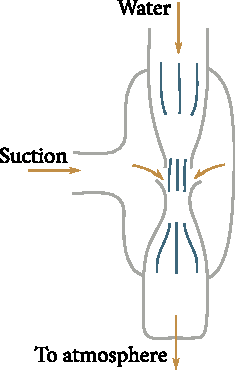
\includegraphics[scale=0.95]{figures/ch_09/fig_9_6.pdf}
		\caption[]{}
		\label{fig:9_6}
	\end{center}
	\vspace{-0.8cm}
\end{figure}

\section{Flow of a Liquid from a Hole}\label{sec:9_3}

Let us apply Bernoulli's equation to the flow of a liquid from a small hole in a wide open vessel. Let us separate in the liquid a flow tube having the open surface of the liquid the vessel as one of its cross sections and the hole through which the liquid flows out\footnote{More exactly, the cross section of the flow emerging front the hole. If special measures are not taken, the section of the Dow will be smaller than the hole.} as the other one (\fig{9_7}). For each of these sections, the velocity and the height above an initial datum level may be considered the same. Consequently, we can apply \eqn{9_4}, obtained on this assumption, to these sections. Further, the pressure in both sections is atmospheric and therefore the same. In addition, the velocity of the open surface in the wide vessel can be assumed to equal zero. With a view to everything said above, \eqn{9_4} can be written in the following form for this case:
\begin{equation*}
	\rho gh_1 = \frac{\rho v^2}{2} + \rho gh_2
\end{equation*}

\noindent
where $v$ is the velocity of the liquid flowing from the hole. Cancelling $p$ and introducing $h=h_1-h_2$, \ie, the height of the open surface of the liquid above the hole, we get $v^2/2=gh$, whence
\begin{equation}\label{eq:9_6}
	v = (2gh)^{1/2}.
\end{equation}

\noindent
This formula is known as the \textbf{Torricelli formula}  (after the Italian physicist Evangelista Torricelli, 1608-1647).

\begin{figure}[t]
	\begin{minipage}[t]{0.5\linewidth}
		\begin{center}
			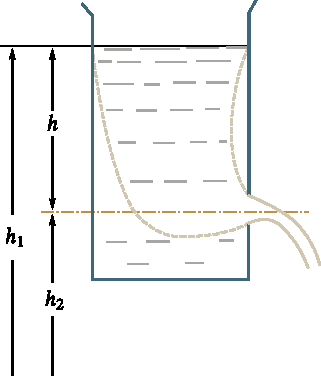
\includegraphics[scale=1.0]{figures/ch_09/fig_9_7.pdf}
			\caption[]{}
			\label{fig:9_7}
		\end{center}
	\end{minipage}
	\hspace{-0.0cm}
	\begin{minipage}[t]{0.5\linewidth}
		\begin{center}
			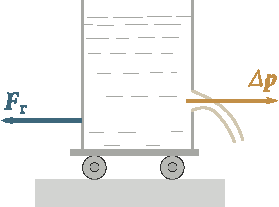
\includegraphics[scale=1.0]{figures/ch_09/fig_9_8.pdf}
			\caption[]{}
			\label{fig:9_8}
		\end{center}
	\end{minipage}
	\vspace{-0.4cm}
\end{figure}

Thus, the velocity with which a liquid is discharged from a hole at a depth of $h$ under an open surface coincides with the velocity which a body acquires in falling from the height $h$. Do not forget that this result was obtained on the assumption that the liquid is ideal. The discharge velocity will be smaller for real liquids, the difference from the value given by \eqn{9_6} growing with an increasing viscosity of the liquid.

A stream of liquid discharged from a hole in a vessel (\fig{9_8}) carries along with it during the time $\Delta t$ the momentum $\Delta\vec{p}=\rho Sv\vec{v}\Delta t$ ($\rho$ is the density of the liquid, $S$ is the cross-sectional area of the hole, $\vec{v}$ is the discharge velocity of the flow). This momentum is imparted to the discharged liquid by the vessel. According to Newton's third law, the vessel receives a momentum equal to $\Delta\vec{p}$ from the discharged liquid during the time $\Delta t$, \ie, experiences the action of the force
\begin{equation}\label{eq:9_7}
	\vec{F}_{\text{r}} = -\frac{\Delta\vec{p}}{\Delta t} = -\rho Sv\vec{v}.
\end{equation}

\noindent
This force is called the \textbf{reaction of the discharged flow} (or the \textbf{thrust}). If our vessel is placed on a cart, then under the action of the force $\vec{F}_{\text{r}}$ it will start moving in the direction opposite to that of the discharged flow.

Let us find the value of the force $\vec{F}_{\text{r}}$ using \eqn{9_6} for the discharge velocity of a liquid from a hole:
\begin{equation}\label{eq:9_8}
	F_{\text{r}} = -\rho Sv^2 = 2gh\rho S.
\end{equation}

\noindent
If, as may seem at first sight, the force $\vec{F}_{\text{r}}$ coincided in magnitude with the force of hydrostatic pressure which the liquid would exert on a plug closing the hole, then $F_{\text{r}}$ would equal $gh\rho S$. The force $\vec{F}_{\text{r}}$ is actually double this value. The explanation is that the motion of the liquid in the vessel appearing when it is discharged leads to redistribution of the pressure, and the pressure near the wall opposite the hole is somewhat greater than near the wall containing the hole.

The operation of jet engines and rockets is based on the reaction or thrust of a discharged gas stream. Reactive motion, not requiring an atmosphere for its accomplishment, is used for flights in outer space.

The outstanding Russian scientist and inventor Konstantin
Tsiolkovsky (1857-1935) founded the theory of interplanetary communications. He presented the theory of a rocket's flight and substantiated the possibility of using jet engines for interplanetary flights. In particular, Tsiolkovsky worked out the theory of motion of composite rockets in which each following stage starts functioning after the preceding stage, having completely used up its fuel, separates from the rocket. Tsiolkovsky's ideas were further developed and realized by Soviet scientists and engineers who ensured the leading role of the Soviet Union in the mastering and studying of outer space.

\section{Forces of Internal Friction}\label{sec:9_4}

An ideal liquid, i.\ie, one without friction, is an abstraction. Viscosity or internal friction is a property inherent to some extent or other in all real fluids (liquids and gases). Viscosity manifests itself in that motion set up in a fluid gradually stops after the action of the reasons causing the motion is discontinued.

Let us consider the following experiment to reveal the laws which forces of internal friction obey. Two parallel plates whose linear dimensions considerably exceed the distance $d$ between them (\fig{9_9}) are immersed in a liquid. The bottom plate is held in place, while the top one is brought into motion relative to the bottom one with a certain velocity $\vec{v}_0$. The experiment shows that to move the top plate with a constant velocity $\vec{v}_0$, we have to exert on it a quite definite force $\vec{F}$ that is constant in magnitude. Since the plate receives no acceleration, this signifies that the action of this force is balanced by a force equal to it in magnitude and opposite in direction which is evidently the force of friction acting on the plate when it moves in the liquid. Let us denote it by $\vec{F}_{\text{fr}}$.

By varying the velocity of the plate $\vec{v}_0$, the area of the plates $S$, and the distance $d$ between them, we can find that
\begin{equation}\label{eq:9_9}
	F_{\text{fr}} = \eta\frac{v_0}{d}S
\end{equation}

\noindent
where $\eta$ is a constant of proportionality depending on the nature and state (for instance, the temperature) of the liquid and called the \textbf{coefficient of internal friction} or the \textbf{viscosity} of the liquid (gas). Sometimes the quantity $\eta$ determined from \eqn{9_9} is called the \textbf{dynamic viscosity} as distinct from the kinematic viscosity $\nu$ equal to $\eta/\rho$, where $\rho$ is the density of the fluid---see Sec.~\ref{sec:9_5}.

\begin{figure}[t]
	\begin{center}
		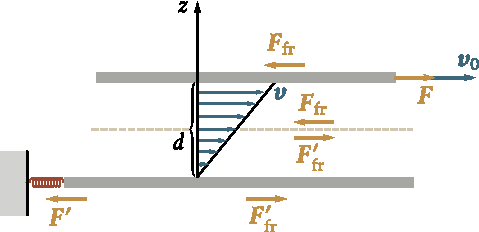
\includegraphics[scale=1.0]{figures/ch_09/fig_9_9.pdf}
		\caption[]{}
		\label{fig:9_9}
	\end{center}
	\vspace{-0.8cm}
\end{figure}

The bottom plate upon motion of the top one also experiences the action of the force $\vec{F}_{\text{fr}}'$ equal in magnitude to $\vec{F}_{\text{fr}}$. For the bottom plate to remain stationary, the force $\vec{F}_{\text{fr}}$ must be balanced with the aid of the force $\vec{F}'$.

Thus, when the two plates immersed in the liquid move relative to each other, interaction characterized by the force~\eqref{eq:9_9} appears between them. The plates obviously act on each other through the liquid between the plates, the force of interaction being transmitted from one layer of the liquid to another. If at any place in the gap between the plates we mentally draw a plane parallel to them (see the dash line in \fig{9_9}), then we can assert that the part of the liquid above this plane acts on the part of the liquid under it with the force $\vec{F}_{\text{fr}}$, and the part of the liquid under the plane, in turn, acts on the part above the plane with the force $\vec{F}_{\text{fr}}$, the values of $\vec{F}_{\text{fr}}$ and $\vec{F}_{\text{fr}}'$ being determined by \eqn{9_9}. Thus, \eqn{9_9} determines not only the force of friction acting on the plates, but also the force of friction between the parts of the liquid in contact.

If we study the velocity of the liquid particles in different layers, it will be found to change in the direction $z$ at right angles to the plates (\fig{9_9}) according to a linear law:
\begin{equation}\label{eq:9_10}
	v(z) = \frac{v_0}{d}z.
\end{equation}

\noindent
The liquid particles in direct contact with the plates adhere to them, as it were, and have the same velocity as the plates themselves. By \eqn{9_10},
\begin{equation}\label{eq:9_11}
	\left|\diff{v}{z}\right| = \frac{v_0}{d}.
\end{equation}

\noindent
We have used the magnitude sign for the following reason. If we had fastened the top plate and moved the bottom one (see \fig{9_9}) or had reversed the direction of the $z$-axis, the derivative $\diffin{v}{z}$ would have become negative. The value of $v_0/d$, however, is always positive. Hence, for \eqn{9_11} to hold in any case, we must take the magnitude of $\diffin{v}{z}$.

Using \eqn{9_11}, we can write \eqn{9_9} as follows:
\begin{equation}\label{eq:9_12}
	F_{\text{fr}} = \eta \left|\diff{v}{z}\right| S.
\end{equation}

This equation determines the magnitude of the force of friction. The quantity $|\diffin{v}{z}|$ shows how fast the velocity changes in the direction of the $z$-axis, and is the magnitude of the gradient of the magnitude of the velocity (if $v$ depends only on $z$, then $\diffinpartial{v}{x}=\diffinpartial{v}{y}=0, \diffinpartial{v}{z}=\diffin{v}{z}$).

We have obtained \eqn{9_12} for the case when the velocity changes according to a linear law. It was found that this equation also holds for any other law of the change in the velocity from layer to layer. In this case to determine the force of friction between two neighbouring layers, we must take the value of $|\diffin{v}{z}|$ at the place where the imaginary interface between the layers passes.

Everything said in this section relates to all fluids.

The unit of viscosity in the SI system is the viscosity at which the gradient of the velocity with a magnitude of \SI{1}{\metre\per\second} per \si{\metre} leads to the appearance of a force of internal friction of \SI{1}{\newton} per \si{\metre\squared} of surface of contact of the layers. This unit is called the \textbf{pascal-second} (\si{\pascal\second})\footnote{The pascal is the name given to the unit of pressure in the SI system ($\SI{1}{\pascal}=\SI{1}{\newton\per\metre\squared}$).}.

The unit of viscosity in the cgs system is the poise (\si{\poise}) equal to the viscosity at which the gradient of the velocity with a magnitude of \SI{1}{\centi\metre\per\second} per \si{\centi\metre} leads to the appearance of a force of internal friction of \SI{1}{\dyne} per \si{\centi\metre\squared} of surface of contact of the layers. The unit equal to \SI{e-6}{\poise} is called the micropoise (\si{\micro\poise}). The poise and the pascal-second are related as follows:
\begin{equation*}
	\SI{1}{\pascal\second} = \SI{10}{\poise}.
\end{equation*}

The viscosity depends on the temperature. The nature of this dependence appreciably differs for liquids and gases. The viscosity of liquids greatly diminishes with increasing temperature. The viscosity of gases, on the contrary, grows with increasing temperature. The difference in the behaviour of $\eta$ with changes in the temperature points to the difference in the mechanism of internal friction in liquids and gases.

\section{Laminar and Turbulent Flows}\label{sec:9_5}

Two kinds of flow of a liquid (or gas) are observed. In some cases, the liquid separates, as it were, into layers that slide relative to one another without mixing. Such flow is called \textbf{laminar} (from the Latin word ``lamina'' meaning plate or strip). If we introduce a coloured stream into a laminar flow, it is retained without being washed out over the entire length of the flow because the liquid particles in a laminar flow do not pass over from one layer to another. A laminar flow is steady.

With an increase in the velocity or cross-sectional dimensions of a flow, its nature changes quite appreciably. Vigorous stirring of the liquid appears. Such a flow is called \textbf{turbulent}. In a turbulent flow, the velocity of the particles at each given place constantly changes chaotically---the flow is not steady. If we introduce a coloured stream into a turbulent flow, already at a small distance from the place of its introduction the coloured liquid will be uniformly distributed over the entire cross section of the flow.

The British scientist Osborne Reynolds (1842-1912) established that the nature of a flow depends on the value of the dimensionless quantity
\begin{equation}\label{eq:9_13}
	\reynolds = \frac{\rho n l}{\eta}
\end{equation}

\noindent
where $\rho$ is the density of the liquid (or gas), $v$ is the average flow velocity (over the cross section of the pipe), $\eta$ is the viscosity of the liquid and $l$ is the dimension characterizing the cross section, for example, the side of the square with a square cross section, the radius or diameter with a round section, etc.

The quantity $\reynolds$ is called the \textbf{Reynolds number}. At small values of the Reynolds number, laminar flow is observed. Beginning from a certain definite value of Re called the critical one, the flow acquires a turbulent nature. If for a round pipe we take its radius $r$ as the characteristic dimension, then the critical value of the Reynolds number (which in this case has the form $\reynolds=\rho vr/\eta$) equals\footnote{It is obvious that if we take the diameter of the pipe instead of its radius as the quantity $l$, we must double the critical value of $\reynolds$.} approximately \num{1000}. The Reynolds number includes the ratio of two quantities depending on the properties of a liquid-the density $\rho$ and the viscosity $\eta$. The ratio
\begin{equation}\label{eq:9_14}
	\nu = \frac{\eta}{\rho}
\end{equation}

\noindent
is called the \textbf{kinematic viscosity}. In contrast to $\nu$, the quantity $\eta$ is known as the \textbf{dynamic viscosity}. Using the kinematic viscosity, we can write the Reynolds number as follows:
\begin{equation}\label{eq:9_15}
	\reynolds = \frac{vl}{\nu}.
\end{equation}

\noindent
The Reynolds number can be used as a dimensionless or similarity number for the flow of liquids in pipes, channels, etc. The nature of the flow of different liquids (or gases) in pipes of different cross sections will be absolutely the same if the same value of $\reynolds$ corresponds to each flow.

\section{Flow of a Liquid in a Round Pipe}\label{sec:9_6}

When a liquid flows through a round pipe, the velocity is zero at the pipe walls and maximum at its axis. Assuming the flow to be laminar, let us find the law of the change in the velocity with the distance $r$ from the pipe axis.

\begin{figure}[t]
	\begin{center}
		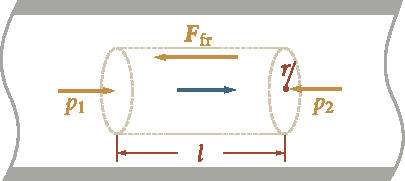
\includegraphics[scale=1.0]{figures/ch_09/fig_9_10.pdf}
		\caption[]{}
		\label{fig:9_10}
	\end{center}
	\vspace{-0.8cm}
\end{figure}

Let us separate an imaginary cylindrical volume of the liquid of radius $r$ and length $l$ (\fig{9_10}). Upon steady flow in a pipe of constant cross section, the velocities of all the particles of the liquid remain unchanged. Hence, the sum of the external forces applied to any volume of the liquid is zero. The bases of the cylindrical volume being considered experience forces of pressure whose sum is $(p_1-p_2)\pi r^2$. This force acts in the direction of motion of the liquid. In addition, the side surface of the cylinder experiences a force of friction equal to $\eta|\diffin{v}{r}|2\pi rl$ (we have in view the value of $\diffin{v}{r}$ at the distance $r$ from the pipe axis). The condition for steady flow has the form
\begin{equation}\label{eq:9_16}
	(p_1 - p_2)\pi r^2 = \eta|\diff{v}{r}|2\pi rl.
\end{equation}

The velocity diminishes with an increasing distance from the pipe axis. Consequently, $\diffin{v}{r}$ is negative, and $|\diffin{v}{r}|=-\diffin{v}{r}$. Taking this into account, we shall transform \eqn{9_16} as follows:
\begin{equation*}
	- \diff{v}{r} = \frac{(p_1 - p_2)r}{2\eta l}.
\end{equation*}

\noindent
Separating the variables, we get
\begin{equation*}
	\deriv{v} = -\frac{(p_1 - p_2)}{2\eta l}r\,\deriv{r}.
\end{equation*}

\noindent
Integration yields
\begin{equation}\label{eq:9_17}
	v = -\frac{(p_1 - p_2)}{4\eta l}r^2 + C
\end{equation}

\noindent
The integration constant must be selected so that the velocity will vanish at the pipe walls, \ie, with $r=R$ ($R$ is the pipe radius). From this condition
\begin{equation*}
	C = \frac{(p_1 - p_2)}{4\eta l}R^2.
\end{equation*}

\noindent
Introduction of the value of $C$ in \eqn{9_17} gives
\begin{equation}\label{eq:9_18}
	v(r) = \frac{(p_1 - p_2)}{4\eta l}\left(R^2 - r^2\right) = \frac{(p_1 - p_2)}{4\eta l}R^2\left(1 - \frac{r^2}{R^2}\right).
\end{equation}

\noindent
The value of the velocity along the axis of the pipe is
\begin{equation}\label{eq:9_19}
	v_0 = v(0) = \frac{(p_1 - p_2)}{4\eta l}R^2.
\end{equation}

\noindent
By using this equation in \eqn{9_18}, we can obtain
\begin{equation}\label{eq:9_20}
	v(r) = v_0 \left(1 - \frac{r^2}{R^2}\right).
\end{equation}

\noindent
Thus, with laminar flow, the velocity changes with an increasing distance from the axis of a pipe according to a parabolic law (\fig{9_11}).

With turbulent flow, the velocity at each point changes chaotically. With constant external conditions, the average (in time) velocity at each point of the cross section of a pipe is constant. The profile of the average velocities in turbulent flow is shown in \fig{9_12}. The velocity changes near the walls of a pipe at a much greater rate than in laminar flow. In the remaining part of the cross section, the change in the velocity is smaller.

\begin{figure}[t]
	\begin{minipage}[t]{0.5\linewidth}
		\begin{center}
			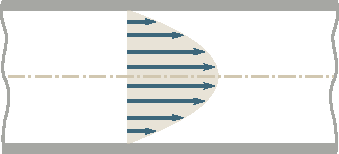
\includegraphics[scale=1.0]{figures/ch_09/fig_9_11.pdf}
			\caption[]{}
			\label{fig:9_11}
		\end{center}
	\end{minipage}
	\hspace{-0.0cm}
	\begin{minipage}[t]{0.5\linewidth}
		\begin{center}
			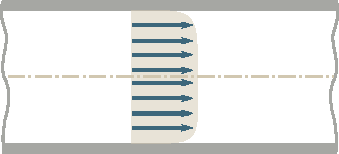
\includegraphics[scale=1.0]{figures/ch_09/fig_9_12.pdf}
			\caption[]{}
			\label{fig:9_12}
		\end{center}
	\end{minipage}
	\vspace{-0.4cm}
\end{figure}

Assuming the flow to be laminar, let us calculate the rate of flow of the liquid $Q$, \ie, the volume of liquid flowing through the cross section of a pipe in unit time. Let us divide the cross section of the pipe into rings with a width of $\deriv{r}$ (\fig{9_13}). In one second, a volume of liquid equal to the product of the ring area $2\pi r\,\deriv{r}$ and the velocity of the flow at the points at a distance of $r$  from the pipe axis will pass through a ring of radius $r$. With a view to \eqn{9_20} we get
\begin{equation}\label{eq:9_21}
	\deriv{Q} = v_0 \left(1 - \frac{r^2}{R^2}\right) 2\pi r\,\deriv{r}.
\end{equation}

\noindent
To obtain the rate of flow $Q$, we must integrate \eqn{9_21} with respect to $r$ within the limits from zero to $R$:
\begin{equation}\label{eq:9_22}
	Q = \int_{0}^{R} v_0 \left(1 - \frac{r^2}{R^2}\right) 2\pi r\,\deriv{r} = \frac{1}{2}\pi R^2 v_0 = \frac{1}{2}Sv_0
\end{equation}

\noindent
($S$ is the cross-sectional area of the pipe). Inspection of \eqn{9_22} shows that in a laminar flow the average value of the velocity (over the cross section) is half the value of the velocity at the axis of the pipe.

\begin{figure}[t]
	\begin{center}
		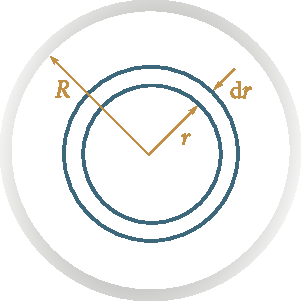
\includegraphics[scale=0.95]{figures/ch_09/fig_9_13.pdf}
		\caption[]{}
		\label{fig:9_13}
	\end{center}
	\vspace{-0.8cm}
\end{figure}

Substituting in \eqn{9_22} the value for $v_0$ from \eqn{9_19}, we get the following formula for the rate of flow:
\begin{equation}\label{eq:9_23}
	Q = \frac{(p_1 - p_2)\pi R^4}{8\eta l}.
\end{equation}

\noindent
This formula is called the \textbf{Poiseuille formula}. According to it, the flow of a liquid is proportional to the pressure drop per unit pipe length, to the fourth power of the pipe radius, and is inversely proportional to the viscosity of the liquid. It must be remembered that the Poiseuille formula may be applied only for a laminar flow.

Formula~\eqref{eq:9_23} is used to determine the viscosity of liquids. By passing a liquid through a capillary of known radius and measuring the pressure drop and the rate of flow $Q$, we can find $\eta$.

\section{Motion of Bodies in Fluids}\label{sec:9_7}

Forces whose resultant will be designated by the symbol $\vec{R}$ (\fig{9_14}) act on a body upon its motion in a fluid\footnote{We shall note that with a constant velocity of a body relative to a fluid the force acting on the body, according to Galileo's principle of relativity, will be the same as when the fluid is moving with the same velocity relative to the stationary body. Figure~\ref{fig:9_14} corresponds to the latter case.}. The force $\vec{R}$ can be resolved into two components, of which $\vec{Q}$ is directed opposite to the motion of the body (or in the direction of the flow advancing onto the body), and $\vec{P}$ at right angles to this direction. The components $\vec{Q}$ and $\vec{P}$ are called the \textbf{drag} (or \textbf{head resistance}) and the \textbf{lift} (or \textbf{lifting force}), respectively. It is obvious that only a drag can act on a body that is symmetrical relative to the direction of motion, while the lift in this case will vanish.

\begin{figure}[t]
	\begin{minipage}[t]{0.4\linewidth}
		\begin{center}
			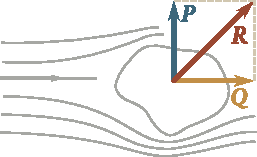
\includegraphics[scale=1.0]{figures/ch_09/fig_9_14.pdf}
			\caption[]{}
			\label{fig:9_14}
		\end{center}
	\end{minipage}
	\hspace{-0.0cm}
	\begin{minipage}[t]{0.6\linewidth}
		\begin{center}
			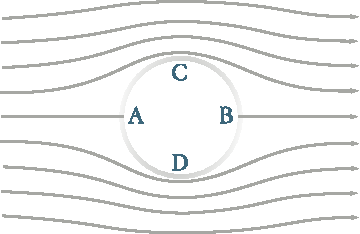
\includegraphics[scale=1.0]{figures/ch_09/fig_9_15.pdf}
			\caption[]{}
			\label{fig:9_15}
		\end{center}
	\end{minipage}
	\vspace{-0.4cm}
\end{figure}

Calculations show that the uniform motion of bodies in an ideal fluid should occur without drag. Having no viscosity, an ideal fluid should slide freely over the surface of a body, flowing completely around it. Figure~\ref{fig:9_15} shows the streamlines when an ideal fluid flows around a very long (``infinite'') cylinder. Owing to complete flowing around the cylinder, the pattern of the streamlines is absolutely symmetrical both relative to the straight line passing through points A and B and relative to the straight line passing through points C and D. Hence, the pressure near points A and B will be the same (and greater than in an undisturbed flow because the velocity near these points is lower). The pressure near points C and D will also be the same (and lower than in an undisturbed flow because the velocity near these points is higher). Consequently, the resultant force of the pressure on the surface of the cylinder (which in the absence of viscosity could set up a drag) will evidently vanish. The same result is also obtained for bodies of a different shape.

Other phenomena are encountered when a body moves in a viscous fluid. In this case, a very thin layer of the fluid adheres to the body's surface and moves together with it as a single whole, carrying along the following layers owing to friction. The velocity of the layers diminishes with an increasing distance from the body's surface and, finally, at a certain distance from the surface the fluid is virtually undisturbed by the motion of the body. The body is thus surrounded by a layer of the fluid in which there is a velocity gradient. This layer is called the \textbf{boundary} one. Friction forces act in it which in the long run are applied to the body and lead to the appearance of a drag. But matters are not exhausted here. The presence of a boundary layer radically changes the nature of the flow of a fluid around a body. Complete flowing around becomes impossible. The action of the friction forces in the surface layer causes the flow to break away from the body's surface. The result is the appearance of eddies behind the body (see \fig{9_16} showing the flow of a viscous fluid around a cylinder). The eddies are carried away by the flow and gradually attenuate owing to friction. The energy of the eddies is spent for heating the fluid. The pressure in the eddy region formed behind the body is lowered. Consequently, the resultant of the pressure forces will differ from zero, this leading in turn to a drag.

The drag thus consists of the friction drag and the pressure drag. With given cross-sectional dimensions of a body, the pressure drag greatly depends on its form. For this reason, it is also called the form drag. Bodies with a well streamlined drop-shaped form (\fig{9_17}) have the smallest pressure drag. Designers do everything possible to impart such a form to the fuselage and wings of aircraft, to the body of motor vehicles, etc.

\begin{figure}[t]
	\begin{minipage}[t]{0.5\linewidth}
		\begin{center}
			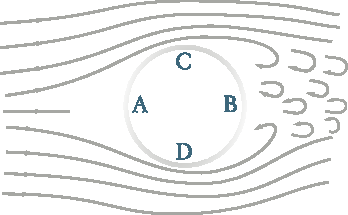
\includegraphics[scale=1.0]{figures/ch_09/fig_9_16.pdf}
			\caption[]{}
			\label{fig:9_16}
		\end{center}
	\end{minipage}
	\hspace{-0.0cm}
	\begin{minipage}[t]{0.5\linewidth}
		\begin{center}
			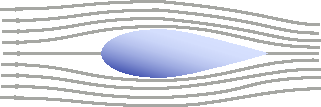
\includegraphics[scale=1.0]{figures/ch_09/fig_9_17.pdf}
			\caption[]{}
			\label{fig:9_17}
		\end{center}
	\end{minipage}
	\vspace{-0.5cm}
\end{figure}

The ratio between the friction drag and the pressure drag is determined by the value of the Reynolds number~\eqref{eq:9_13}. Here, $l$ is a characteristic dimension of the body in question (for example, the radius for a spherical body), and $v$ is the velocity of the body relative to the fluid.

At small values of $\reynolds$, the main part is played by the friction drag, so that the pressure drag may be disregarded. The part of the pressure drag grows more and more with increasing $\reynolds$. At great values of $\reynolds$, pressure forces predominate in the drag.

When determining the nature of the forces acting on a body in a flow, the Reynolds number can be used as a similarity number (scale factor) in this case too. This circumstance is taken advantage of in modelling. For example, a model of an aeroplane will behave in a gas flow the same as the full-scale counterpart if in addition to geometrical similarity of the model and the aeroplane, the Reynolds number will also be equal for them.

\textbf{The Stokes Formula.} At small values of $\reynolds$, \ie, at low velocities [and small $l$'s, see \eqn{9_13}], the resistance of a medium is due virtually only to the friction forces. George Stokes (1819-1903) established that the drag force in this case is proportional to the dynamic viscosity $\eta$, the velocity $v$ of a body relative to the fluid, and the characteristic dimension of the body $l$, \ie $F\propto\eta lv$ (it is assumed that the distance from the body to the boundaries of the fluid, for example, to the walls of a vessel confining it, considerably exceeds the dimensions of the body). The proportionality constant depends on the form of the body. For a sphere, if we take its radius $r$ as the dimension $l$, the proportionality constant is $6\pi$. Hence, the drag force on a sphere in fluids at small velocities, according to the Stokes formula, is
\begin{equation}\label{eq:9_24}
	F = 6\pi\eta rv.
\end{equation}

\textbf{Lift.} The viscosity of a fluid is of no significance for the appearance of a lift. Figure~\ref{fig:9_18} shows the streamlines when an ideal fluid flows around a half-cylinder. Owing to complete flowing around, the streamlines will be symmetrical relative to straight line CD. The pattern will not be symmetrical, however, relative to straight line AB. The streamlines are closer together near point C, therefore the pressure here will be lower than near point D, and the lift $\vec{P}$ appears. A lift appears similarly in a viscous fluid.

\begin{figure}[t]
	\begin{minipage}[t]{0.5\linewidth}
		\begin{center}
			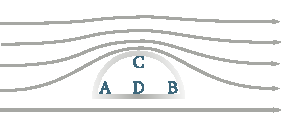
\includegraphics[scale=1.0]{figures/ch_09/fig_9_18.pdf}
			\caption[]{}
			\label{fig:9_18}
		\end{center}
	\end{minipage}
	\hspace{-0.1cm}
	\begin{minipage}[t]{0.5\linewidth}
		\begin{center}
			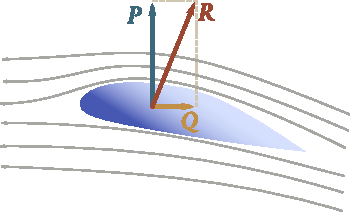
\includegraphics[scale=1.0]{figures/ch_09/fig_9_19.pdf}
			\caption[]{}
			\label{fig:9_19}
		\end{center}
	\end{minipage}
	\vspace{-0.5cm}
\end{figure}

The force keeping an aeroplane in the air is the lift acting on its wings. The drag is harmful during the flight of an aeroplane. This is why the wings of an aeroplane and its fuselage are given a well streamlined shape. The profile of an aerofoil (wing) must also ensure an adequate lift. The profile shown in \fig{9_19}, found by the outstanding Russian scientist Nikolai Zhukovsky (1847-1921) is the optimal one for an aerofoil. The works of Zhukovsky and his pupil S. Chaplygin laid the foundation of modern aerodynamics. V. Lenin called Zhukovsky the father of Russian aviation. Zhukovsky, in particular, derived a formula for determining the lift that is the basis of all aerodynamic calculations of aeroplanes.
